\documentclass[a4paper,12pt,oneside,openany,table,xcdraw]{article}

\usepackage{setspace}
\usepackage{multirow}
\usepackage{hyperref}
\usepackage{caption}
\usepackage{indentfirst}
\usepackage{tikz} %% fasores
\usetikzlibrary{arrows,arrows.meta,quotes,angles}
\usepackage{siunitx}

\usepackage[brazilian]{babel}
\usepackage[utf8x]{inputenc}
\usepackage{amsmath, graphicx, subfig, enumerate}
\usepackage{float, verbatim}
\usepackage[colorinlistoftodos]{todonotes}
\usepackage{makeidx}
\usepackage{geometry}

\graphicspath{{img/}}
\geometry{a4paper, hmargin={3cm, 3cm}, vmargin={3cm, 2cm} }
\setlength{\parindent}{1.0cm}
\captionsetup{font=small}

\usepackage{mathtools,listings} %%
\usepackage{color} %red, green, blue, yellow, cyan, magenta, black, white
\definecolor{mygreen}{RGB}{28,172,0} % color values Red, Green, Blue
\definecolor{mylilas}{RGB}{170,55,241}
\usepackage{listingsutf8}

\begin{document}
\newcommand{\thedepartment}{Faculdade de Engenharia Elétrica}
\newcommand{\thecourse}{FEELT}
\newcommand{\thetitle}{Resolução da Lista de Exercícios Extras}
\newcommand{\thetype}{Trabalho de Sinais e Sistemas II}
\newcommand{\theproftitle}{Bacharel em Engenharia Elétrica}
\newcommand{\thestudent}{Lesly Viviane Montúfar Berrios\\
\centering11811ETE001}
\newcommand{\theadvisor}{Prof. Wellington Maycon Santos Bernardes}
\newcommand{\thecity}{Uberlândia}

\thispagestyle{empty}\newcommand*{\themonth}{\ifthenelse{\the\month < 2}{Janeiro }
                  {\ifthenelse{\the\month < 3}{Fevereiro }
                  {\ifthenelse{\the\month < 4}{Março }
                  {\ifthenelse{\the\month < 5}{Abril }
                  {\ifthenelse{\the\month < 6}{Maio }
                  {\ifthenelse{\the\month < 7}{Junho }
                  {\ifthenelse{\the\month < 8}{Julho }
                  {\ifthenelse{\the\month < 9}{Agosto }
                  {\ifthenelse{\the\month < 10}{Setembro }
                  {\ifthenelse{\the\month < 11}{Outubro }
                  {\ifthenelse{\the\month < 12}{Novembro }{Dezembro }}}}}}}}}}}}
                  
\begin{titlepage}
\begin{center}

	\vspace{-0.5cm}

  \begin{figure}[hbt!]
		\begin{center}
		   
\includegraphics[width=2.8cm]{ufu-logo.png}
		\end{center}
	\end{figure}
 	%\vspace{-4cm}

%\begin{doublespacing}

  \Large{\textbf{Universidade Federal de Uberlândia}}\\
  \large{\thedepartment}\\
  \large{\thecourse}\\


\vspace{5.8cm}
  \par
  \large\textbf{\thetitle}
\vspace{5.8cm} 

%\end{doublespacing}
  \par
  \thetype\\
  por\\
  %\hspace{2cm}\large{}\\

\vspace{0.8cm}
\par
  \normalsize{\thestudent}\\ [2cm]
  \theadvisor

\par\vfill
  \thecity, \themonth / \the\year

\end{center}

\end{titlepage}

\lstset{language=Matlab,%
	inputencoding=utf8/latin1,
    %basicstyle=\color{red},
    breaklines=true,%
    morekeywords={matlab2tikz},
    keywordstyle=\color{blue},%
    morekeywords=[2]{1}, keywordstyle=[2]{\color{black}},
    identifierstyle=\color{black},%
    stringstyle=\color{mylilas},
    commentstyle=\color{mygreen},%
    showstringspaces=false,%without this there will be a symbol in the places where there is a space
    numbers=left,%
    numberstyle={\tiny \color{black}},% size of the numbers
    numbersep=9pt, % this defines how far the numbers are from the text
    emph=[1]{for,end,break},emphstyle=[1]\color{red}, %some words to emphasise
    %emph=[2]{word1,word2}, emphstyle=[2]{style},    
}

%% Comeca o documento !

\onehalfspacing
\tableofcontents % sumário
\newpage

\section{Exercício 1}
 Por meio do código em anexo (Anexo \ref{anexo:ex1}) foi possível as informações retirar informações dispostas nas subssões seguintes.
\vspace{0.3cm}

% \lstinputlisting{EX1/EX1.m}

\vspace{0.3cm}
\subsection{Determinação de polos e zeros e curva de resposta em frequência}
Pede-se modelar um filtro seletivo para uma determinada frequência $f_rejeitada$, da qual se extrairá os polos e zeros necessários. Para isso, é necessário relacionar a frequência a ser retirada com a frequência de amostragem $F_S$ por meio de $w_{rejeitada} = 2*pi*freq_{rejeitada}/F_s$, da qual se retira os os zeros $0.5877 - 0.8089i$ e $0.5877 + 0.8089i$, e polos $0.0823 - 0.2427i$,  $0.0823 + 0.2427i$,  $0.3703 - 0.6067i$ e $0.3703 + 0.6067i$. Na Figura \ref{ex1:polos} tem-se o diagrama de polos correspondente do filtro projetado.

\vspace{0.6cm}
\begin{figure}[H]
\centering
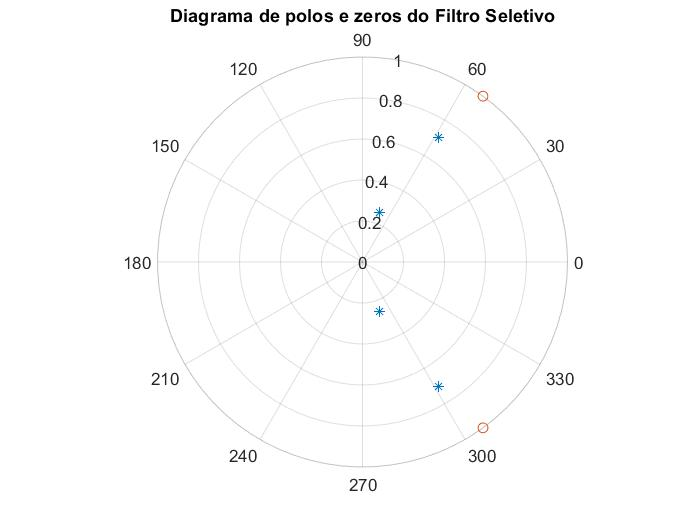
\includegraphics[width=13cm]{ex1-pz}
\caption{Diagramas de polos e zeros do filtro seletivo.}
\label{ex1:polos}
\end{figure}
\vspace{0.4cm}

A partir dos polos e zeros é possível plotar a curva da resposta em frequência, como na Figura \ref{ex1:H}. Dela vê-se que tem-se o propósito de atenuar a frequência digital de $\dfrac{3 \pi}{10}$.
\vspace{0.4cm}

\begin{figure}[H]
\centering
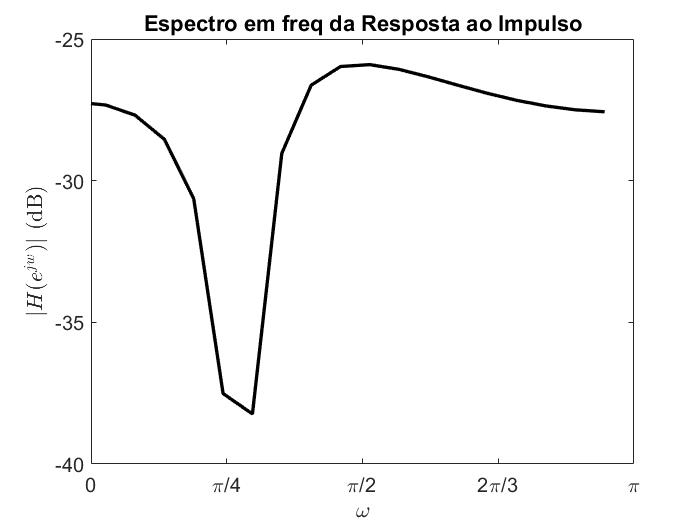
\includegraphics[width=13cm]{ex1-h}
\caption{Resposta em frequência do filtro seletivo.}
\label{ex1:H}
\end{figure}
\vspace{0.1cm}

\subsection{Equação de diferenças e taxa de aquisição}



\section{Anexos}
\subsection{Código correspondente ao exercício 1} \label{anexo:ex1}
\lstinputlisting{EX1/EX1.m}

\subsection{Código correspondente ao exercício 2} \label{anexo:ex2}
\lstinputlisting{EX1/EX1.m}

\subsection{Código correspondente ao exercício 3} \label{anexo:ex3}
\lstinputlisting{EX1/EX1.m}

\subsection{Código correspondente ao exercício 4} \label{anexo:ex4}
\lstinputlisting{EX1/EX1.m}

\newpage
\begin{thebibliography}{9} 
% Introdução
\bibitem{S1}
    ...,
    “Sistemas de Controle para a Engenharia”, Avaliação da Qualidade da Energia Elétrica, DSE – FEEC – UNICAMP , 2019.
 
\bibitem{S2}
    ...,
    “Sinais e Sistemas”,... , 2019.

\end{thebibliography}
\end{document}
